\section{Class Diagrams}

\begin{figure}[h!]
    \centering
    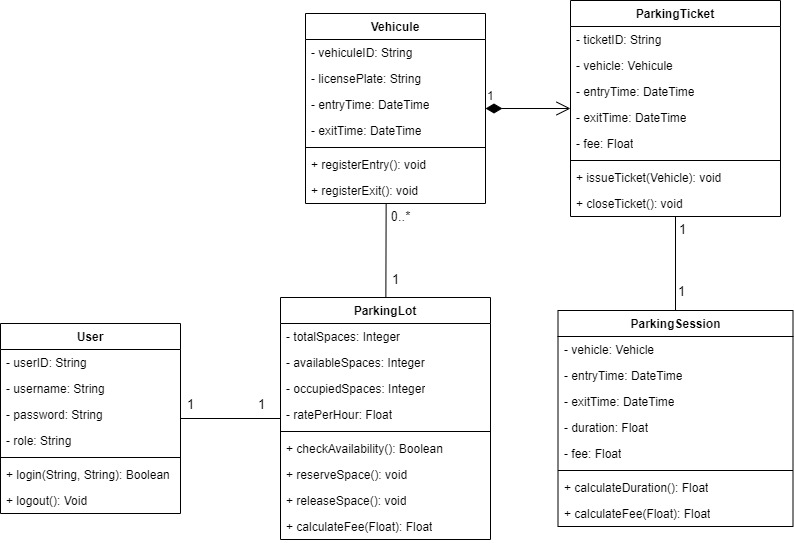
\includegraphics[width=1\textwidth]{Class_Diagram_Parkinglot_System.jpg} % Ruta al archivo PDF con el diagrama
    \caption{UML Class Diagram for the Parking Management System}
    \label{fig:uml}
\end{figure}

This system consists of the following classes:

\begin{enumerate}
    \item \textbf{User (Admin)}
    \item \textbf{Vehicle}
    \item \textbf{ParkingTicket}
    \item \textbf{ParkingLot}
    \item \textbf{ParkingSession}
\end{enumerate}

Each class has certain attributes and methods, and the relationships between them are defined as follows.

\subsection{Classes and Their Details}

\subsubsection{User Class}
The \textbf{User} class represents the administrator who manages the parking lot operations.

\subsubsection*{Attributes}
\begin{itemize}
    \item \texttt{userID (String)}: A unique identifier for the user (e.g., "admin001").
    \item \texttt{username (String)}: The username used to log into the system.
    \item \texttt{password (String)}: The password for the user account.
    \item \texttt{role (String)}: The role of the user (typically "admin").
\end{itemize}

\subsubsection*{Methods}
\begin{itemize}
    \item \texttt{login(username: String, password: String): Boolean}: Verifies the login credentials. Returns \texttt{true} if the login is successful, otherwise returns \texttt{false}.
    \item \texttt{logout(): void}: Logs the user out of the system.
\end{itemize}

\subsubsection{Vehicle Class}
The \textbf{Vehicle} class represents a vehicle entering or exiting the parking lot.

\subsubsection*{Attributes}
\begin{itemize}
    \item \texttt{vehicleID (String)}: A unique identifier for the vehicle (e.g., "V001").
    \item \texttt{licensePlate (String)}: The license plate number of the vehicle.
    \item \texttt{entryTime (DateTime)}: The time when the vehicle enters the parking lot.
    \item \texttt{exitTime (DateTime)}: The time when the vehicle exits the parking lot.
\end{itemize}

\subsubsection*{Methods}
\begin{itemize}
    \item \texttt{registerEntry(): void}: Records the entry time of the vehicle.
    \item \texttt{registerExit(): void}: Records the exit time of the vehicle.
\end{itemize}

\subsubsection{ParkingTicket Class}
The \textbf{ParkingTicket} class represents a ticket issued when a vehicle enters the parking lot.

\subsubsection*{Attributes}
\begin{itemize}
    \item \texttt{ticketID (String)}: A unique identifier for the parking ticket (e.g., "T001").
    \item \texttt{vehicle (Vehicle)}: The vehicle associated with this ticket.
    \item \texttt{entryTime (DateTime)}: The entry time of the vehicle.
    \item \texttt{exitTime (DateTime)}: The exit time of the vehicle.
    \item \texttt{fee (Float)}: The parking fee based on the vehicle's duration in the lot.
\end{itemize}

\subsubsection*{Methods}
\begin{itemize}
    \item \texttt{issueTicket(vehicle: Vehicle): void}: Issues a parking ticket when a vehicle enters the parking lot.
    \item \texttt{closeTicket(): void}: Closes the ticket and calculates the parking fee based on the duration.
\end{itemize}

\subsubsection{ParkingLot Class}
The \textbf{ParkingLot} class represents the parking lot itself and manages parking spaces.

\subsubsection*{Attributes}
\begin{itemize}
    \item \texttt{totalSpaces (Integer)}: The total number of spaces in the parking lot.
    \item \texttt{availableSpaces (Integer)}: The number of available spaces in the parking lot.
    \item \texttt{occupiedSpaces (Integer)}: The number of spaces occupied by vehicles.
    \item \texttt{ratePerHour (Float)}: The parking rate per hour.
\end{itemize}

\subsubsection*{Methods}
\begin{itemize}
    \item \texttt{checkAvailability(): Boolean}: Returns \texttt{true} if there are available spaces, otherwise \texttt{false}.
    \item \texttt{reserveSpace(): void}: Reserves a space when a vehicle enters the parking lot.
    \item \texttt{releaseSpace(): void}: Releases a space when a vehicle exits the parking lot.
    \item \texttt{calculateFee(duration: Float): Float}: Calculates the parking fee based on the duration the vehicle stayed.
\end{itemize}

\subsubsection{ParkingSession Class}
The \textbf{ParkingSession} class tracks the duration and fee for a vehicle's parking session.

\subsubsection*{Attributes}
\begin{itemize}
    \item \texttt{vehicle (Vehicle)}: The vehicle associated with the parking session.
    \item \texttt{entryTime (DateTime)}: The entry time of the vehicle.
    \item \texttt{exitTime (DateTime)}: The exit time of the vehicle.
    \item \texttt{duration (Float)}: The duration in hours the vehicle was parked.
    \item \texttt{fee (Float)}: The parking fee for the session.
\end{itemize}

\subsubsection*{Methods}
\begin{itemize}
    \item \texttt{calculateDuration(): Float}: Calculates the duration of the vehicle's stay, in hours, between entry and exit times.
    \item \texttt{calculateFee(ratePerHour: Float): Float}: Calculates the fee based on the duration and rate per hour.
\end{itemize}

\subsection{Relationships Between Classes}

\subsubsection{User $<->$ ParkingLot}
The \textbf{User} class (admin) interacts with the \textbf{ParkingLot} class to view and manage the parking lot's statistics and vehicle entries and exits.

\subsubsection*{Relationship Type}
\begin{itemize}
    \item \textbf{Association}: The admin interacts with the parking lot but does not own it.
    \item \textbf{Multiplicity}: 1 \texttt{User} $<->$ 1 \texttt{ParkingLot} (one user can manage one parking lot).
\end{itemize}

\subsubsection{Vehicle $<->$ ParkingTicket}
The \textbf{Vehicle} class is associated with the \textbf{ParkingTicket} class, which tracks the vehicle's entry and exit times.

\subsubsection*{Relationship Type}
\begin{itemize}
    \item \textbf{Composition}: A parking ticket cannot exist without the vehicle it is assigned to.
    \item \textbf{Multiplicity}: 1 \texttt{Vehicle} $<->$ 1 \texttt{ParkingTicket} (each vehicle has exactly one parking ticket).
\end{itemize}

\subsubsection{ParkingLot $<->$ Vehicle}
The \textbf{ParkingLot} class manages multiple vehicles, and each vehicle occupies one parking space.

\subsubsection*{Relationship Type}
\begin{itemize}
    \item \textbf{Association}: The parking lot can contain multiple vehicles.
    \item \textbf{Multiplicity}: 1 \texttt{ParkingLot} $<->$ 0..* \texttt{Vehicle} (a parking lot can contain multiple vehicles, but a vehicle is in only one parking lot at a time).
\end{itemize}

\subsubsection{ParkingTicket $<->$ ParkingSession}
The \textbf{ParkingTicket} class is associated with the \textbf{ParkingSession} class, which tracks the duration and fee of the parking session.

\subsubsection*{Relationship Type}
\begin{itemize}
    \item \textbf{Association}: Each parking ticket has one associated parking session.
    \item \textbf{Multiplicity}: 1 \texttt{ParkingTicket} $<->$ 1 \texttt{ParkingSession} (one ticket has exactly one parking session).
\end{itemize}
